\chapter{Preliminaries}\label{approach}

Before talking about the inference rules, some preliminary notations need to be established. First, the notion of a \textit{callsite} seems at its first glance trivial but becomes more complex when considering references that may contain callsites or again references to other callsite-containing tables. Second, the effect of shadowing must be formally captured. Third, some simplifying notations and placeholders are introduced to shorten the already lenghtly rules.

\section{Subset of SQL}
%\begin{verbatim}
%[ WITH with_query [, ...] ]
%SELECT [ ALL | DISTINCT [ ON ( expression [, ...] ) ] ]
%    [ * | expression [ [ AS ] output_name ] [, ...] ]
%    [ FROM from_item [, ...] ]
%    [ WHERE condition ]
%
%where from_item can be one of:
%    table_name [ * ] [ [ AS ] alias [ ( column_alias [, ...] ) ] ]
%    ( select ) [ AS ] alias [ ( column_alias [, ...] ) ]
%    with_query_name [ [ AS ] alias [ ( column_alias [, ...] ) ] ]
%    function_name ( [ argument [, ...] ] ) [ AS ] alias ( column_definition [, ...] )
%    from_item [ NATURAL ] join_type from_item [ ON join_condition | USING ( join_column [, ...] ) ]
%
%and with_query is:
%    with_query_name [ ( column_name [, ...] ) ] AS ( select | values )
%\end{verbatim}

%\setlength{\grammarparsep}{20pt plus 1pt minus 1pt} % increase separation between rules
%\setlength{\grammarindent}{12em} % increase separation between LHS/RHS 

\begin{figure}[H]
    \begin{minted}{postgresql}
    <query>     ::= [ WITH (<query>) AS <tblAlias>[, ...] ]
                      SELECT [ DISTINCT ] <expr>  AS <colAlias>[, ...]
                    [ FROM <tbl>     AS <tblAlias>[, ...] ]
                    [ WHERE <expr> ]
                 |  <query> <qfun> <query>
    <tbl>       ::= <tblRef> | (<query>) | <fun>([<expr>, ...])
    <expr>      ::=  <const> |  <colRef> |  <fun>([<expr>, ...])
                 |  CASE [WHEN <expr> THEN <expr>, ...] ELSE <expr> END
                 |  ( <query> )
    <fun>       ::= UDFs and sql built-in operators, functions, aggregates that are stable
    <qfun>      ::= UNION [ALL]
    <const>     ::= sql built-in constants
    <tblAlias>  ::= alias(colAlias[, ...])
    <colAlias>  ::= alias
    \end{minted}
    \caption{The subset of SQL we consider throughout this thesis.}
    \label{lst:sql_grammar}
\end{figure}


%\subsection{No VOLATILE functions}
%Without referential transparancy we cannot assume that two function calls within the same query return the same value, making it impossible to use memoization. Therefore, only UDFs markes as STABLE or IMMUTEABLE (38.7. Function Volatility Categories) are translateable.
%Since we use \texttt{UNION} during the evaluation-phase, the rows are checked on equality. This confronts us with a quirk of PostgreSQL: Composite types have no built in function to check equality, thus \texttt{UNION} fails while checking if two composite-types are equal. Later on we will lift this constraint by casting the nonhashable types to and from text.

%Normal UNION require sortable or hashable, but in WITH RECURSIVE it is always hashable, see\footnote{https://www.postgresql-archive.org/Hashable-custom-types-td5801576.html, https://www.postgresql.org/docs/10/static/xindex.html#XINDEX-OPCLASS-DEPENDENCIES, }

\section{Notation}
We say a subtree in the query-block of an UDF named $fn$ has or contains a callsite, if and only if the tree contains a node with a call to the function itself or contains a reference to a table that has a callsite. This table in turn does not need to contain an explicit recursive call but can also contain a reference to a table that is recursive by this definition. This comes from the property that table-references are transitive.
\\\\
\section{Semantic equivalence of UDFs}
Equivalence for mathematical functions is intuitively defined as $f: S \mapsto T, g: U \mapsto V, \forall x \in S: f(x) = g(x)$ with $S = U, T = V$. If the domain, ie. the function signature, matches and the results are equal for every input, the functions are considered to be equivalent. We have to extend this definition a little to bear the newly introduced aspects of real (database-)world procedures.

The signatures of a PostgreSQL-UDF does contain many different keywords reflecting properties of the function to give hints to the database-system how to UDF is callable or what kind of optimizations are applicable. Therefore, we require the translation not only to match the function signature (say: $gcd(int, int) : int$), but also the complete CREATE FUNCTION-block surrounding the actual function body. If a function is marked eg. as IMMUTABLE, the translation preserves this property. The only exception are UDFs that are marked PARALLEL SAFE, that is changed to PARALLEL RESTRICTED since the translation uses non-parallel safe operations like CTE-Scans (15.4. Parallel Safety).

In general, we cannot assume that UDFs are total, ie. that they terminate for all possible inputs from the input space. Assume a function that only terminates for positive inputs or may throw a division-by-zero error. This behaviour must be preserved by the translation, otherwise it would be not be clear if an error is actual a bug in the original function or introduced by the translation.

RETURNS NULL ON NULL INPUT\\
VARIADIC (argument list)\\
DEFAULTs\\
argmodes?\\
positional vs named notation: breaks calls!


\section{Auxillary notations}
\begin{align*}
    T[a \mapsto \top] &:= T \cup \{a\}\\
    T[a \mapsto \bot] &:= T \setminus \{a\}\\
    T[a_1 \mapsto r_1, ..., a_n \mapsto r_n] &:= T[a_1 \mapsto r_1] \cdots[a_n \mapsto r_n]\\
\end{align*}
\\\\
For the CTE-store $C$ we define an ordered hash-map with the CTE-alias $a$ as key. The empty CTE-store is denoted as $\varnothing$. A new CTE, given by the CTE-body $t$, its predicate $p$ and the set of referenced CTEs on the same level $r$, is specified as $e=(t, p, r)$ alongside with its key $a$. It is appended to $C$ by the following operation: $C[a: e]$. Ordered subsets of $C$ can be retrieved by filtering for matching keys, ignoring keys not found: $C[\{a_1, ..., a_n, a_x\}] = \langle (a_1, t_1, p_1, r_1)_1, \dots, (a_n, t_n, p_n, r_n)_n\rangle$.
\\\\
The auxiliary function $\sigma_{\text{cols}}$ is used to pick columns from the store by name, eg. $\sigma_{a, t, p, r}(C)$ returns the entire store $\langle (a, t, p, r)_1, \dots, (a, t, p, r)_n \rangle$ and $\sigma_p(C) = \langle p_1, \dots, p_n \rangle$ all predicates in the store.
\\\\


\chapter{Analysis rules}

The data structure which is generated by the inference rules is a tuple $(B, R)$. $B$ and $R$ are sets of scenarios. Each scenario is again a tuple of the scenario predicate and the scenario query.

$$
\Big(
    \overbrace{\big\{
        \underbrace{
            (p_1, q_1)
        }_{\text{scenario 1}}
    \big\}}^{\text{basecase scenarios}}
    ,
    \overbrace{\big\{
        \underbrace{
            (p_2, q_2)
        }_{\text{scenario 2}},
        \underbrace{
            (p_3, q_3)
        }_{\text{scenario 3}}
    \big\}}^{\text{recursive scenarios}}
\Big)
$$


$$\quad(\textsc{base})\inferrule{
   T \vdash \neg \hasCallsite(e) \\
   \neg \text{isElse}(e)
}{
    T, \varnothing \vdash (p, e) \rightarrow (\{(p, e)\},\{\})
}$$
\\
% REC
$$\quad(\textsc{rec})\inferrule{
   \forall i \in \{1, ..., n\} : T \vdash \neg \hasCallsite(x_i)
}{
    T, C \vdash (p, fn(x_1, ..., x_n)) \rightarrow (\{\}, \{(p, fn(x_1, ..., x_n))\})
}$$
% REF
$$\quad(\textsc{ref})\inferrule{
   \text{isReference}(S) \\
   T \vdash \hasCallsite(S)
}{
    T, C \vdash (p, S) \rightarrow (\{\}, \{(p, S)\})
}$$
\\

In the following section I will present inference rules to extract relevant features from the UDF that are needed to choose an appropiate template and fill it accordingly. As we allow callsites only in the S-F-W part of a query, the rules only covers them explicitly. Nevertheless, keywords like DISTINCT, ORDER BY, LIMIT, OFFSET etc. are also meant to be covered by the rules, but would disgrade readability greatly.

Before stating the inference rules it is necessary to formalize some terminology and introduce notations that will help us keeping the rules comprehensible.


Inference rules are applied to compute the first intermediate representation of the original query. They are given in the form of an Small-Step Operational Semantics and lead to a tuple $(B, R)$ that holds semantically equivalent versions of the original query under certain constraints of the arguments. These constraints are conjunctions of the predicates used in the (maybe nested) \CASE-expressions of the query. They are given as formula $p$ in propositional logic alongside with the pruned query (resp. expression) $q$. Is a pruned query nonrecursive, the tuple is element $B$, otherwise element $R$.
\\\\

To understand shadowing in SQL, ie. overriding a previous definition of a variable inside the current scope, we first need to understand what scopes are created in different parts of a query. CTEs and table-definitions inside the FROM-part of a query can create new table-references. For each CTE, the scope is the following query, including following CTEs. An CTE is available in every part of the following query, including \FROM. Table-references created inside the \FROM-part of the query are not visible to other, sibling talbe-references from the same \FROM. CTEs are evaluated before query execution, so the \FROM-scope is below the \WITH-scope, ie. CTEs can be overriden from table-references by the \FROM-part of the same query. \footnote{Note the difference between \textit{table}-references (\texttt{T}), that are solely established inside \FROM and \WITH, and \textit{table-row}-references ($\texttt{T.v}$) that access table-references in other parts of the query.} Furthermore, each subquery creates its own scope, potentially overriding outer table-references.
\\\\
Explain T and C
\\\\
There are two base-rules that require no more rule application and lead to an immidiate result: \RBASE and \RREC. The \RBASE-rule is applicable when a subtree $q$ contains no recursive calls or references to recursive table-expressions. We directly obtain the resulting tuple $(\{q\}, \emptyset)$. The other case is the \RREC-rule, which handles a subtree $q$ where the root node is the recursive call itself. To comply with the overall restrictions given under X.Y.Z, no argument may have a callsite. If this is given, the rule leads directly to $(\emptyset, \{q\})$. TODO: EXPLAN REF
\\\\
All other rules require a callsite somewhere within the query, unwrapping each layer of the query until the callsite is reached or no callsite exists in the subtree. The rules for handling \CASE-statements create for each possible outcome one pruned version while extending the given predicate by the predicate of the taken \WHEN-branch. In contrast to SELECT-statements and CASE-expressions, other parts of the query \textit{can} contain callsites in sibling subtrees. The idea here is to compute all possible outcomes of these subtrees independantly and then build the cartesian-product to receive all possible scenarios of the execution of the parent node. The \REXPR-rule implements purely this idea and the \RCTE and \RFROM-rule come as variations or extensions that take distinct particularities into account.
\\\\
The most complicated rule is for handling \WITH-statements. As in the \REXPR-rule, each execution-scenario for every CTE is computed and then the cartesion-product is build over all the scanarios. But two difficulties needs to be considered: First, each CTE can reference previous CTEs from within the same WITH-statement. Second, not every CTE may be referenced later on when the actually query (without the CTEs) is processed - eg. the referencing part may be pruned away after application of a \RWHEN-rule. This leads to to multiple identical versions of the original query that only differ in their predicates, namely by the case-distinctions from the unused CTE. This is semantically not a problem but can degrade performance, since callsites are enumerated based on the set of recursive and nonrecursive cases. Unfortunately, it is hardly possible to postpone this step to postprocessing since we would have to identify and remove the parts caused by the unused CTE from the predicate. Thus we hve two rules for handling CTEs: One for processing and removing each CTE one by one from the query and one for reconstructing the original \WITH-Statement, limited to that CTEs that are actually used by the translated query eventually.
\\\\
So, how does the CTE-Rules work in detail? Each CTE is processed on its own, one by one. The processed CTE is removed from the query and put into the variable-store and added alongside with its predicate to the temporary CTE-list. Depending on the processed CTE the recursive or nonrecursive store/list is choosen. Computation continues as long as CTEs are present. Finally, the complete query including CTEs is reconstructed. The actual query is translated with emptied temporary CTE-lists. Only CTEs that are referenced (directly or indirectly) are kept and their predicates are appended to the result predicate. To find out what CTEs are referenced, all free variables under the given environment need to be recursivly followed.

\section{Handling case distinctions}
The case distinctions made by \CASE-Statements are the actual language construct we are interested in. They introduce the differenct scenarios that we want to extract. The \WHEN-part establishes the \textit{predicate} of the \textit{result} inside the \THEN-part of each branch. Each consecutive \WHEN implies the negation of all previous \WHEN's. Our task here is to factor out this implicit negations into standaline predicates that could be evaluated as set of simple \texttt{IF}s.

In the following, I visualize the logical program flow in a diagrams. An arrow to the right means that the predicate is fulfilled, an arrow down denotes the negation. Predicates $p$ are surrounded by a single lined border while doubled bordered box marks the result $r$ of the \CASE-statement. An asteriks $\ast$ marks recursive subexpressions.

\subsection{Simple \CASE-distinctions with recursive \THEN's only}
Previous predicates are negated and stacked up.

\setlength{\tabcolsep}{2pt}
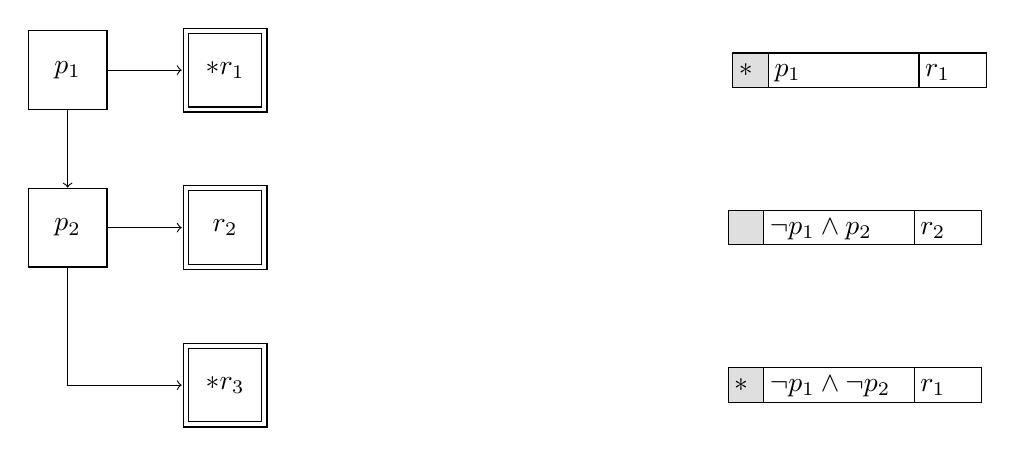
\begin{tikzpicture}[x=20mm, y=20mm]
\tikzset{Pred/.style={shape=rectangle, draw, minimum width=1cm, minimum height=1cm}}
\tikzset{Res/.style={shape=rectangle, draw, double distance=0.5mm, outer sep=0.5mm, minimum width=1cm, minimum height=1cm}}

% nodes
\node[Pred] (p1) at (0, 2) {$p_1$};
\node[Res]  (r1) at (1, 2) {$\ast r_1$};
\node (case1) at (5, 2) {
{}
\begin{tabular}{|p{3mm}|p{5em}|p{2em}|}\hline
\cellcolor{gray!25} $\ast$ & $p_1$ & $r_1$\\\hline
\end{tabular}};

\node[Pred] (p2) at (0, 1) {$p_2$};
\node[Res] (r2) at (1, 1) {$r_2$};
\node (case1) at (5, 1) {\begin{tabular}{|p{3mm}|p{5em}|p{2em}|}\hline
\cellcolor{gray!25} ~~ & $\neg p_1 \land p_2$ & $r_2$\\\hline
\end{tabular}};

\node[Res] (r3) at (1, 0) {$\ast r_3$};
\node (case1) at (5, 0) {\begin{tabular}{|p{3mm}|p{5em}|p{2em}|}\hline
\cellcolor{gray!25} $\ast$ & $\neg p_1 \land \neg p_2$ & $r_1$\\\hline
\end{tabular}};
% arrows
\draw[->] (p1) -> (r1);
\draw[->] (p1) -- (p2);
\draw[->] (p2) -- (r2);
\draw[->] (p2) |- (r3);
\end{tikzpicture}

\iffalse
\begin{tabular}{|r|rrr|r|}\hline
$\ast$ &      $p_1$ &         &            & $r_1$ \\\hline
       & $\neg p_1$ & $\land$ &      $p_2$ & $r_2$ \\\hline
$\ast$ & $\neg p_1$ & $\land$ & $\neg p_2$ & $r_3$      \\\hline
\end{tabular}
\fi

\subsection{Recursive \WHEN's}
Recursive predicates cannot be solved and are therefore considered as part of the result (recursive) expression. Slicing stops before a recursive predicate.

\begin{tikzpicture}[x=20mm, y=20mm]
\tikzset{Pred/.style={shape=rectangle, draw, minimum width=1cm, minimum height=1cm}}
\tikzset{Res/.style={shape=rectangle, draw, double distance=0.5mm, outer sep=0.5mm, minimum width=1cm, minimum height=1cm}}

% nodes
\node[Pred] (p1) at (0, 1.5) {$p_1$};
\node[Res]  (r1) at (1, 1.5) {$r_1$};
\node at (5, 1.5) {\begin{tabular}{|p{3mm}|p{5em}|p{2em}|}\hline
\cellcolor{gray!25} & $p_1$ & $r_1$\\\hline
\end{tabular}};

\node[Res, inner sep=3mm] (res) at (0.5, 0) {
    \begin{tikzpicture}[x=20mm, y=20mm, inner sep=1em]
        \node[Pred] (p2) at (0, 1) {$\ast p_2$};
        \node[Pred] (r2) at (1, 1) {$r_2$};
        \node[Pred] (r3) at (1, 0) {$r_3$};
        \draw[->] (p2) -- (r2);
        \draw[->] (p2) |- (r3);
    \end{tikzpicture}
};
\node at (5, 0) {\begin{tabular}{|c|c|c|}\hline
\cellcolor{gray!25} $\ast$ & $\neg p_1$ & $\WHEN ~p_2~ \THEN ~r_1~ \ELSE ~r_3$\\\hline
\end{tabular}};
% arrows
\draw[->] (p1) -> (r1);
\draw[->] (p1) -> (0, 0.95);
\end{tikzpicture}

\subsection{Nonrecursive subtrees}
Subtrees with no callsite are taken as one big basecase without further slicing.

\begin{tikzpicture}[x=20mm, y=20mm]
\tikzset{Pred/.style={shape=rectangle, draw, minimum width=1cm, minimum height=1cm}}
\tikzset{Res/.style={shape=rectangle, draw, double distance=0.5mm, outer sep=0.5mm, minimum width=1cm, minimum height=1cm}}

% nodes
\node[Pred] (p1) at (0, 1.5) {$p_1$};
\node[Res]  (r1) at (1, 1.5) {$\ast r_1$};
\node at (5, 1.5) {\begin{tabular}{|p{3mm}|p{5em}|p{2em}|}\hline
\cellcolor{gray!25} $\ast$ & $p_1$ & $r_1$\\\hline
\end{tabular}};

\node[Res, inner sep=3mm] (res) at (0.5, 0) {
    \begin{tikzpicture}[x=20mm, y=20mm, inner sep=1em]
        \node[Pred] (p2) at (0, 1) {$p_2$};
        \node[Pred] (r2) at (1, 1) {$r_2$};
        \node[Pred] (r3) at (1, 0) {$r_3$};
        \draw[->] (p2) -- (r2);
        \draw[->] (p2) |- (r3);
    \end{tikzpicture}
};
\node at (5, 0) {\begin{tabular}{|c|c|c|}\hline
\cellcolor{gray!25} ~~ & $\neg p_1$ & $\WHEN ~p_2~ \THEN ~r_1~ \ELSE ~r_3$\\\hline
\end{tabular}};
% arrows
\draw[->] (p1) -> (r1);
\draw[->] (p1) -> (0, 0.95);
\end{tikzpicture}

\subsection{Nested Case in \THEN}
Predicates stack up linearily when nested inside \THEN.

\begin{tikzpicture}[x=15mm, y=15mm]
\tikzset{Pred/.style={shape=rectangle, draw, minimum width=1cm, minimum height=1cm}}
\tikzset{Box/.style={shape=rectangle, draw, minimum width=1cm, minimum height=1cm, dotted, very thick}}
\tikzset{Res/.style={shape=rectangle, draw, double distance=0.5mm, outer sep=0.5mm, minimum width=1cm, minimum height=1cm}}

% nodes
\node[Pred] (p) at (0, 1) {$p$};
\node[Box]  (r1) at (2, 1) {
    \begin{tikzpicture}[x=15mm, y=15mm]
        \node[Pred] (p1) at (0, 2.5) {$p_1$};
        \node[Res] (r1) at (1, 2.5) {$r_1$};
        
        \node[Pred] (pi) at (0, 1) {$p_i$};
        \node[Res] (ri) at (1, 1) {$r_i$};
        % arrows
        \draw[->] (p1) -- (r1);
        \draw[->] (pi) -- (ri);
        \draw[->, dash pattern=on 5pt off 1pt on 3pt off 3pt on 1pt off 2pt on 1pt off 2pt on 3pt off 1pt] (p1) -- (pi);
        \draw[->, dash pattern=on 5pt off 1pt on 3pt off 3pt on 1pt off 2pt on 1pt off 2pt on 3pt off 1pt] (pi) -- +(0,-1);
    \end{tikzpicture}
};
\node at (5, 2) {
    \begin{tabular}{|p{1em}|p{3cm}|c|}\hline
    \cellcolor{gray!25}  & $p \land \phantom{\neg}p_1 $& $r_1$\\\hline
    \end{tabular}
};
   
\node at (5, 1.4) { 
    \vdots
};
    
\node at (5, 0.65) {
    \begin{tabular}{|p{1em}|p{3cm}|c|}\hline
    \cellcolor{gray!25}  & $p \land \neg p_1 \land \neg p_2 \land \hdots \land p_i$& $r_2$\\\hline
    \end{tabular}
};
% arrows
\draw[->] (p) -- (r1);
\end{tikzpicture}


\iffalse
\begin{tabular}{lllrrrrrrrrrr}
\WHEN ~$p_1$~ \THEN & &                        &         $r_1$&  &$\Rightarrow$ (&     $p_1$ &       &           &         &               &                    &, $r_1$)\\
\WHEN ~$p_2$~ \THEN &(&\WHEN ~$p_{2,1}$~ \THEN &     $r_{2,1}$&  &$\Rightarrow$ (&$\neg p_1$ &$\land$&     $ p_2$& $\land$ &    $ p_{2,1}$ &                    &, $r_{2,1}$)\\
                    & &\WHEN ~$p_{2,2}$~ \THEN &     $r_{2,2}$&  &$\Rightarrow$ (&$\neg p_1$ &$\land$&     $ p_2$& $\land$ &$\neg p_{2,1}$ &                    &, $r_{2,2}$)\\
                    & &\ELSE                   &$\ast r_{2,3}$&) &$\Rightarrow$ (&$\neg p_1$ &$\land$&     $ p_2$& $\land$ &$\neg p_{2,1}$ &$\land \neg p_{2,2}$&, $r_{2,1}$)\\
\ELSE               & &                        &    $\ast r_3$&  &$\Rightarrow$ (&$\neg p_1$ &$\land$& $\neg p_2$&         &               &                    &, $r_3$)\\
\end{tabular}
\fi


\subsection{Nested Case in \WHEN's}
When \CASE-expressions are nested inside \WHEN, there two ways not to receive a given result.

\begin{tikzpicture}[x=15mm, y=15mm]
\tikzset{Pred/.style={shape=rectangle, draw, minimum width=1cm, minimum height=1cm}}
\tikzset{Box/.style={shape=rectangle, draw, minimum width=1cm, minimum height=1cm, dotted, very thick}}
\tikzset{Res/.style={shape=rectangle, draw, double distance=0.5mm, outer sep=0.5mm, minimum width=1cm, minimum height=1cm}}


% nodes
\node[Pred] (p) at (0, 3) {$p$};

\node[Box] (p1) at (0, 1) {
    \begin{tikzpicture}[x=15mm, y=15mm]
        \node[Pred] (p2) at (0, 1) {$\pi_i$};
        \node[Pred] (r2) at (1, 1) {$p_i$};
        % arrows
        \draw[->] (p2) -- (r2);
        \draw[->] (r2) -- +(0, -1);
        \draw[<-, dash pattern=on 5pt off 1pt on 3pt off 3pt on 1pt off 2pt on 1pt off 2pt on 3pt off 1pt] (p2) -- +(0,1);
        \draw[->, dash pattern=on 5pt off 1pt on 3pt off 3pt on 1pt off 2pt on 1pt off 2pt on 3pt off 1pt] (p2) -- +(0,-1);
    \end{tikzpicture}
};
\node[Res] (r1) at (2, 1) {$\ast r_i$};
\node (case1) at (4, 1) {
    \begin{tabular}{|p{1em}|r|c|}\hline
    \cellcolor{gray!25} $\ast$ & $\neg p \land \pi_i \land p_i$ & $r_i$\\\hline
    \end{tabular}
};

\node[Res] (r) at (0, -1) {$\ast r$};
\node (case1) at (4, -1) {
    \begin{tabular}{|p{1em}|rrr|c|}\hline
    \cellcolor{gray!25} $\ast$ & $\neg p \land$ & $     \pi_i$ & $\land \neg p_i$ & $r$\\\hline
    \cellcolor{gray!25} $\ast$ & $\neg p \land$ & $\neg \pi_i$ &                  & $r$\\\hline
    \end{tabular}
};
% arrows
\draw[->] (p) -- (p1);
\draw[->] (p1) -- (r1);
\draw[->] (p1) -- (r);
\end{tikzpicture}

\subsection{\CASE- and \ELSE-rules}
\begin{prooftree}
    \AxiomC{}\RightLabel{\scriptsize(base)}
    \UnaryInfC{\lstinputlisting{snippets/rules/fib/03-case-when.sql}}
    \AxiomC{}\RightLabel{\scriptsize(base)}
    \UnaryInfC{\lstinputlisting{snippets/rules/fib/03-case-then.sql}}
    \AxiomC{\vdots}\RightLabel{\scriptsize(else)}
    \UnaryInfC{\lstinputlisting{snippets/rules/fib/03-case-else.sql}}
    \RightLabel{\scriptsize(when)}
    \TrinaryInfC{\lstinputlisting{snippets/rules/fib/02-case.sql}}
\end{prooftree}


$$\quad(\textsc{when})\inferrule{
    \neg (\hasCallsite(p) \land \hasCallsite(bs))\\
    T, C \vdash (\TRUE, p) \rightarrow (B_p, R_p) \\
    T, C \vdash (\TRUE, e) \rightarrow (B_e, R_e)\\
    B_p = \{(p_{p_1}, p'_1), ..., (p_{p_n}, p'_n)\} \\
    \forall (p_{p_i}, p'_i) \in B_p: T, C \vdash (p_0 ~\AND~ p_{p_i}~\AND~\NOT~ p'_i,~ \CASE bs \END) \rightarrow (B_i, R_i) \\
}{
    T, C \vdash (p_0, \CASE \WHEN p \THEN e ~bs \END) \rightarrow \\\\
    {\begin{tabular}[b]{LLLLLL}
        (&\{&(p_0 ~\AND~ p_p ~\AND~ p' ~\AND~ p_e &, e'&) ~|~~(p_p, p') \in B_p, (p_e, e') \in B_e \} &~\cup~ (\cup_{1\leq i \leq n}B_i), \\
         &\{&(p_0 ~\AND~ p_p ~\AND~ p' ~\AND~ p_e &, e'&) ~|~~(p_p, p') \in B_p, (p_e, e') \in R_e \}&~\cup~ (\cup_{1\leq i \leq n}R_i) ~\cup \\
         &\{&(p_0 ~\AND~ p_p ~\AND~ p_0             &, \CASE \WHEN p'_1 \THEN e ~bs \END&) ~|~~(p_p, p') \in R_p \})
    \end{tabular}}
}$$

$$\quad(\textsc{else})\inferrule{
    T, C \vdash (p, e) \rightarrow (B, R) \\
}{
    T, C \vdash (p, \CASE \ELSE e \END) \rightarrow (B, R)
}$$

\section{Handling recursive operands}

\begin{figure}
    \centering
    \footnotesize
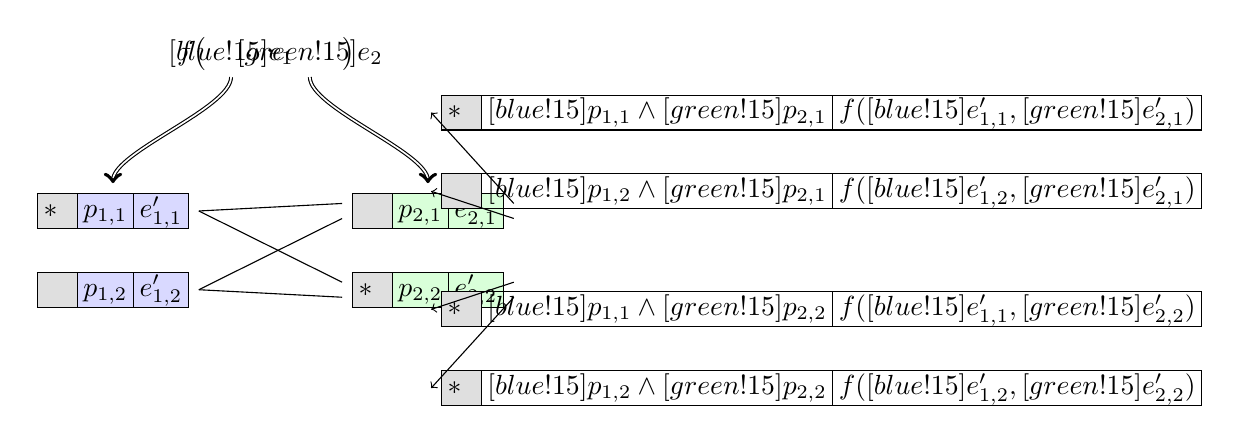
\begin{tikzpicture}[x=10mm, y=10mm]
\node      at (1, 5) {$f\big($};
\node (e1) at (1.5, 5) {$\highlight[blue!15]{e_1}$};
\node      at (2, 5) {$,$};
\node (e2) at (2.5, 5) {$\highlight[green!15]{e_2}$};
\node      at (3, 5) {$\big)$};

\node (e11) at (0, 3) { 
    \begin{tabular}{|p{1em}|r|c|}\hline
    \cellcolor{gray!25} $\ast$ & \cellcolor{blue!15}${p_{1,1}}$ & \cellcolor{blue!15}${e'_{1,1}}$\\\hline
    \end{tabular}
};
\node (e12) at (0, 2) { 
    \begin{tabular}{|p{1em}|r|c|}\hline
    \cellcolor{gray!25}  & \cellcolor{blue!15}${p_{1,2}}$ & \cellcolor{blue!15}${e'_{1,2}}$\\\hline
    \end{tabular}
};

\node (e21) at (4, 3) { 
    \begin{tabular}{|p{1em}|r|c|}\hline
    \cellcolor{gray!25}  & \cellcolor{green!15}${p_{2,1}}$ & \cellcolor{green!15}${e'_{2,1}}$\\\hline
    \end{tabular}
};
\node (e22) at (4, 2) { 
    \begin{tabular}{|p{1em}|r|c|}\hline
    \cellcolor{gray!25}$\ast$ & \cellcolor{green!15}${p_{2,2}}$ & \cellcolor{green!15}${e'_{2,2}}$\\\hline
    \end{tabular}
};

\node (r1) at (9, 4.25) { 
    \begin{tabular}{|p{1em}|r|c|}\hline
    \cellcolor{gray!25} $\ast$ & $\highlight[blue!15]{p_{1,1}} \land \highlight[green!15]{p_{2,1}}$ & $f(\highlight[blue!15]{e'_{1,1}}, \highlight[green!15]{e'_{2,1}})$\\\hline
    \end{tabular}
};
\node (r2) at (9, 3.25) { 
    \begin{tabular}{|p{1em}|r|c|}\hline
    \cellcolor{gray!25}  & $\highlight[blue!15]{p_{1,2}} \land \highlight[green!15]{p_{2,1}}$ & $f(\highlight[blue!15]{e'_{1,2}}, \highlight[green!15]{e'_{2,1}})$\\\hline
    \end{tabular}
};

\node (r3) at (9, 1.75) { 
    \begin{tabular}{|p{1em}|r|c|}\hline
    \cellcolor{gray!25} $\ast$ & $\highlight[blue!15]{p_{1,1}} \land \highlight[green!15]{p_{2,2}}$ & $f(\highlight[blue!15]{e'_{1,1}}, \highlight[green!15]{e'_{2,2}})$\\\hline
    \end{tabular}
};
\node (r4) at (9, 0.75) { 
    \begin{tabular}{|p{1em}|r|c|}\hline
    \cellcolor{gray!25} $\ast$ & $\highlight[blue!15]{p_{1,2}} \land \highlight[green!15]{p_{2,2}}$ & $f(\highlight[blue!15]{e'_{1,2}}, \highlight[green!15]{e'_{2,2}})$\\\hline
    \end{tabular}
};
\draw[->, double, out=270, in=90, looseness = 0.5] (e1.south) to (e11);
\draw[->, double, out=270, in=90, looseness = 0.5] (e2.south) to (e21);

\draw (e11.east) -- (e21.175);
\draw (e11.east) -- (e22.175);
\draw (e12.east) -- (e21.185);
\draw (e12.east) -- (e22.185);

\draw[->] (e21.5) -- (r1.west);
\draw[->] (e21.355) -- (r2.west);
\draw[->] (e22.5) -- (r3.west);
\draw[->] (e22.355) -- (r4.west);
\end{tikzpicture}

    \caption{Operands of a function are translated separately. For each operand a number of scenarios is generated. All possible scenarios of the original function are created by using the cross product.}
    \label{fig:expr-expr}
\end{figure}

\subsection{Single recursive operand}
\subsection{Multiple recursive operands}
\subsection{EXPR-Rule}
$
\inferrule*[Right=(expr)]{
    \inferrule*[Left=(rec)]{ }{
        {\begin{minipage}[b]{15em}
        \mintinline{postgresql}{(TRUE, fib($1 - 1)) ->}
        \mintinline{postgresql}{({}, {(TRUE, fib($1 - 1))})}
        \end{minipage}}
    }\\
    \inferrule*[Right=(rec)]{ }{
        {\begin{minipage}[b]{15em}
        \mintinline{postgresql}{(TRUE, fib($1 - 2)) ->}
        \mintinline{postgresql}{({}, {(TRUE, fib($1 - 2))})}
        \end{minipage}}
    }
}{
    {\begin{minipage}[b]{25em}
    \mintinline{postgresql}{(TRUE, fib($1 - 1) + fib($1 - 2)) ->}
    \mintinline{postgresql}{({}, {(TRUE AND TRUE AND TRUE, fib($1 - 1) + fib($1 - 2))})}
    \end{minipage}}
}
$

$$\quad(\textsc{expr})\inferrule{
    \exists i \in \{1, ..., n\}: T \vdash \hasCallsite(e_i)\\
    \forall i \in \{1, ..., n\}: T, C \vdash (\TRUE, e_i) \rightarrow (B_i, R_i)
}{
    T, C \vdash (p, \oplus_{1\leq i \leq n} e_i) \rightarrow \\\\
    {\begin{tabular}[b]{LLL}
        (&\{(p ~\AND~ (\AND_{1\leq i \leq n} p_i)), \oplus_{1\leq i \leq n} e_i' &~|~~ ((p_1, e_1'), ..., (p_n, e_n')) \in \times_{\{i|1\leq i \leq n\}} ~B_i\}, \\
        &\{(p ~\AND~ (\AND_{1\leq i \leq n } p_i)), \oplus_{1\leq i \leq n} e_i &~|~~ ((p_1, e_1'), ..., (p_n, e_n')) \in \times_{\{i|1\leq i \leq n\}} (B_i \cup R_i),\\&&~~~~\exists e \in \{e'_1, ..., e'_n\} : \hasCallsite(T, e)\})
    \end{tabular}}
}$$
\\


\subsection{\RSELECT- and \RFROM-rule}
\begin{figure}
    \centering
    {\small
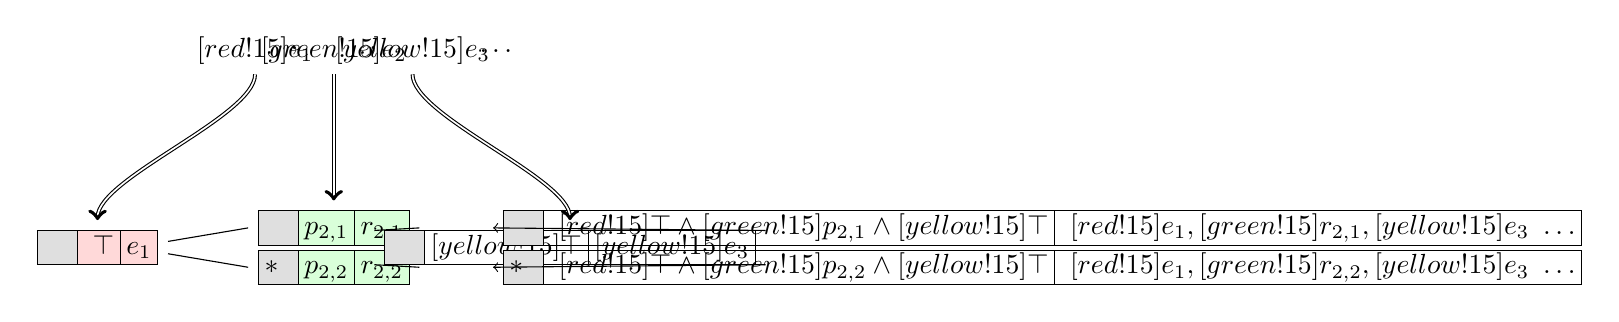
\begin{tikzpicture}[x=5mm, y=5mm]
\node      at ( 8, 9) {$\SELECT$};
\node (e1) at (10, 9) {$\highlight[red!15]{e_1}$};
\node      at (11, 9) {$,$};
\node (e2) at (12, 9) {$\highlight[green!15]{e_2}$};
\node      at (13, 9) {$,$};
\node (e3) at (14, 9) {$\highlight[yellow!15]{e_3}$};
\node      at (16, 9) {$\FROM ~ \dots$};

\node (e11) at (6, 4) { 
    \begin{tabular}{|p{1em}|r|c|}\hline
    \cellcolor{gray!25}  & \cellcolor{red!15} $\top$ & \cellcolor{red!15}$e_1$\\\hline
    \end{tabular}
};

\node (e21) at (12, 4.5) { 
    \begin{tabular}{|p{1em}|r|c|}\hline
    \cellcolor{gray!25}  & \cellcolor{green!15}$p_{2,1}$ & \cellcolor{green!15}$r_{2,1}$\\\hline
    \end{tabular}
};
\node (e22) at (12, 3.5) { 
    \begin{tabular}{|p{1em}|r|c|}\hline
    \cellcolor{gray!25} $\ast$ & \cellcolor{green!15}$p_{2,2}$ & \cellcolor{green!15}$r_{2,2}$\\\hline
    \end{tabular}
};

\node (e31) at (18, 4) { 
    \begin{tabular}{|p{1em}|r|c|}\hline
    \cellcolor{gray!25} & $\highlight[yellow!15]{\top}$ & $\highlight[yellow!15]{e_3}$\\\hline
    \end{tabular}
};

\node (r1) at (30, 4.5) { 
    \begin{tabular}{|p{1em}|r|c|}\hline
    \cellcolor{gray!25}  & $\SELECT ~ \highlight[red!15]{\top} \land \highlight[green!15]{p_{2,1}} \land \highlight[yellow!15]{\top}$ & $\SELECT~ \highlight[red!15]{e_1}, \highlight[green!15]{r_{2,1}}, \highlight[yellow!15]{e_3} ~ \FROM \dots$\\\hline
    \end{tabular}
};
\node (r2) at (30, 3.5) { 
    \begin{tabular}{|p{1em}|r|c|}\hline
    \cellcolor{gray!25} $\ast$ & $\SELECT ~ \highlight[red!15]{\top} \land \highlight[green!15]{p_{2,2}} \land \highlight[yellow!15]{\top}$ & $\SELECT~ \highlight[red!15]{e_1}, \highlight[green!15]{r_{2,2}}, \highlight[yellow!15]{e_3} ~ \FROM \dots$\\\hline
    \end{tabular}
};
\draw[->, double, out=270, in=90, looseness = 0.5] (e1.south) to (e11);
\draw[->, double, out=270, in=90, looseness = 0.5] (e2.south) to (e21);
\draw[->, double, out=270, in=90, looseness = 0.5] (e3.south) to (e31);
\draw (e11.5) to (e21.west);
\draw (e11.355) to (e22.west);
\draw (e21.east) to (e31.175);
\draw (e22.east) to (e31.185);
\draw[->] (e31.5) -- (r1.west);
\draw[->] (e31.355) -- (r2.west);
%\draw[->, bend left=20]  (e11.north) to (e21.north) to (e31.north) to (r1.west);
%\draw[->, bend right=20] (e11.south) to (e22.south) to (e31.south) to (r2.west);
\end{tikzpicture}}
    \caption{The projection of a relation happening inside \SELECT~can be viewed as a function with a number of operands, ie. the output columns. The same happens analogiously for the \FROM-clause.}
    \label{fig:expr-select}
\end{figure}

\subsection{\RSELECT- and \RFROM-rule}
\begin{figure}
    \centering
    {\small
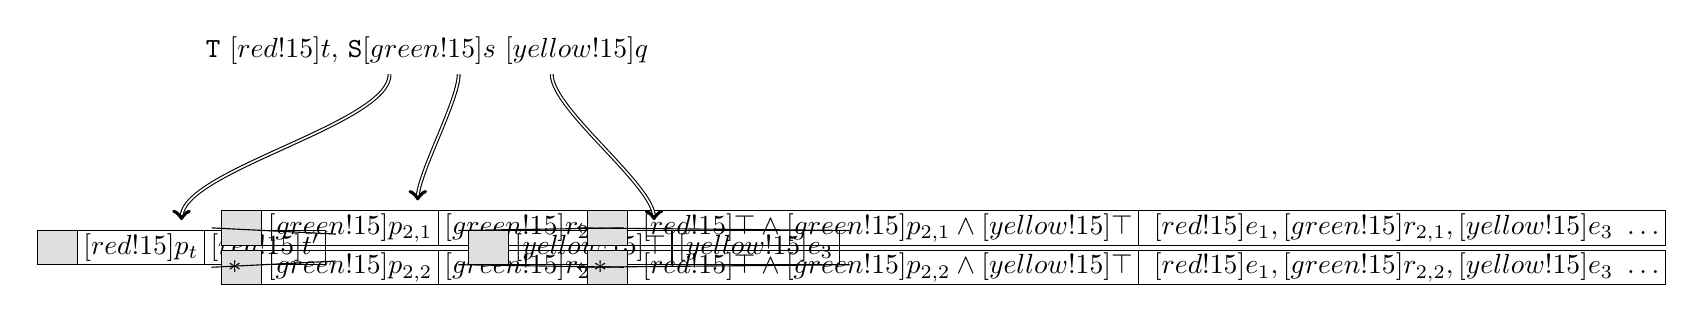
\begin{tikzpicture}[x=5mm, y=5mm, node distance=1mm]
\node (ctes) at (12,9) {\WITH~ \texttt{T} \AS $\highlight[red!15]{t}$, \texttt{S}\AS $\highlight[green!15]{s}$ $\highlight[yellow!15]{q}$};

\node (e11) at (6, 4) { 
    \begin{tabular}{|p{1em}|r|c|}\hline
    \cellcolor{gray!25}  & $\highlight[red!15]{p_t}$ & $\highlight[red!15]{t'}$\\\hline
    \end{tabular}
};

\node (e21) at (12, 4.5) { 
    \begin{tabular}{|p{1em}|r|c|}\hline
    \cellcolor{gray!25}  & $\highlight[green!15]{p_{2,1}}$ & $\highlight[green!15]{r_{2,1}}$\\\hline
    \end{tabular}
};
\node (e22) at (12, 3.5) { 
    \begin{tabular}{|p{1em}|r|c|}\hline
    \cellcolor{gray!25} $\ast$ & $\highlight[green!15]{p_{2,2}}$ & $\highlight[green!15]{r_{2,2}}$\\\hline
    \end{tabular}
};

\node (e31) at (18, 4) { 
    \begin{tabular}{|p{1em}|r|c|}\hline
    \cellcolor{gray!25} & $\highlight[yellow!15]{\top}$ & $\highlight[yellow!15]{e_3}$\\\hline
    \end{tabular}
};

\node (r1) at (30, 4.5) { 
    \begin{tabular}{|p{1em}|r|c|}\hline
    \cellcolor{gray!25}  & $\SELECT ~ \highlight[red!15]{\top} \land \highlight[green!15]{p_{2,1}} \land \highlight[yellow!15]{\top}$ & $\SELECT~ \highlight[red!15]{e_1}, \highlight[green!15]{r_{2,1}}, \highlight[yellow!15]{e_3} ~ \FROM \dots$\\\hline
    \end{tabular}
};
\node (r2) at (30, 3.5) { 
    \begin{tabular}{|p{1em}|r|c|}\hline
    \cellcolor{gray!25} $\ast$ & $\SELECT ~ \highlight[red!15]{\top} \land \highlight[green!15]{p_{2,2}} \land \highlight[yellow!15]{\top}$ & $\SELECT~ \highlight[red!15]{e_1}, \highlight[green!15]{r_{2,2}}, \highlight[yellow!15]{e_3} ~ \FROM \dots$\\\hline
    \end{tabular}
};
\draw[->, double, out=270, in=90, looseness = 0.5] (ctes.220) to (e11);
\draw[->, double, out=270, in=90, looseness = 0.5] (ctes.330) to (e21);
\draw[->, double, out=270, in=90, looseness = 0.5] (ctes.350) to (e31);
\draw (e11.5) to (e21.west);
\draw (e11.355) to (e22.west);
\draw (e21.east) to (e31.175);
\draw (e22.east) to (e31.185);
\draw[->] (e31.5) -- (r1.west);
\draw[->] (e31.355) -- (r2.west);
%\draw[->, bend left=20]  (e11.north) to (e21.north) to (e31.north) to (r1.west);
%\draw[->, bend right=20] (e11.south) to (e22.south) to (e31.south) to (r2.west);
\end{tikzpicture}}
    \caption{The projection of a relation happening inside \SELECT~can be viewed as a function with a number of operands, ie. the output columns. The same happens analogiously for the \FROM-clause.}
    \label{fig:expr-select}
\end{figure}

If the callsites of a query a located in the \FROM-part, it means that at least one table referenced is recursive, ie. contains a callsite or a reference a recursive table. 
As the tables within the same \FROM cannot reference each other, we can process each table independently and resemble the whole query with all possible combinations, similar to the \REXPR-rule. For an example see this example:
\sqlcode[mathescape=true]{snippets/rule_from_example.sql}


$
\inferrule*{
    \inferrule*{...}{
{\begin{minipage}[b]{12em}
\sqlcode{snippets/rules/fib/01-case.sql}
\end{minipage}}
    }
}{
{\begin{minipage}[b]{12em}
\sqlcode{snippets/rules/fib/01-select.sql}
\end{minipage}}
}
$


$$\quad(\textsc{select})\inferrule{
    \exists i \in \{1, ..., k\}: T \vdash \hasCallsite(e_{s_i}) \\
    \forall i \in \{1 \leq i \leq n\} : T \vdash \neg \hasCallsite(e_{t_i}) \\
    T \vdash \neg \hasCallsite(e_{w}) \\
    \forall i \in \{1, ..., k\}: T, \varnothing \vdash (\TRUE, e_{s_i}) \rightarrow (B_i, R_i)
}{
    T, \varnothing \vdash (p, \SELECT [\texttt{DISTINCT}]~ e_{s_1}, ..., e_{s_k} \FROM t_1 \AS a_1 \otimes ... \otimes  t_n \AS a_n \WHERE e_w) \rightarrow \\\\
    {\begin{tabular}[b]{LLLL}
    (~~&\{&(&\SELECT p ~\AND~ p_{s_1} ~\AND~ \cdots ~\AND~ p_{s_k},\\
        &&&\SELECT [\texttt{DISTINCT}]~ e'_{s_1}, ..., e'_{s_k} \FROM t_1 \AS a_1 \otimes ... \otimes  t_n \AS a_n \WHERE e_w~~) \\
        && | &~((p_{s_1}, e'_{s_1}), ..., (p_{s_k}, e'_{s_k})) \in \times_{1 \leq i \leq k} B_i~~\}, \\
     &\{&(&\SELECT p ~\AND~ p_{s_1} ~\AND~ \cdots ~\AND~ p_{s_k}, \\
        &&&\SELECT [\texttt{DISTINCT}]~ e'_{s_1}, ..., e'_{s_k} \FROM t_1 \AS a_1 \otimes ... \otimes  t_n \AS a_n \WHERE e_w~~) \\
        && | &~((p_{s_1}, e'_{s_1}), ..., (p_{s_k}, e'_{s_k})) \in \times_{1 \leq i \leq k} (B_i \cup R_i), \exists e \in \{e'_{s_1}, ..., e'_{s_k}\} : \hasCallsite(e)~~\}~~)\\
    \end{tabular}}
}$$
\subsection{WHERE-Rule}
$$\quad(\textsc{where})\inferrule{
    T \vdash \neg \hasCallsite(e_{s}) \\
    \forall i \in \{1 \leq i \leq n\} : T \vdash \neg \hasCallsite(e_{t_i}) \\
    T \vdash \hasCallsite(e_{w}) \\
    T, \varnothing \vdash (p, e_{w}) \rightarrow (B, R)
}{
    T, \varnothing \vdash (p, \SELECT e_s \FROM t_1 \AS a_1 \otimes ... \otimes  t_n \AS a_n \WHERE e_w) \rightarrow \\\\
    {\begin{tabular}[b]{LLLL}
    (~~&\{&(&\SELECT p_w  \FROM t_1 \AS a_1 \otimes ... \otimes  t_n \AS a_n \WHERE e'_w,\\
        &&&\SELECT e_s \FROM t_1 \AS a_1 \otimes ... \otimes  t_n \AS a_n \WHERE e'_w~~) \\
        && | &~(p_w, e'_w) \in B~~\}, \\
     &\{&(&\SELECT p_w \FROM t_1 \AS a_1 \otimes ... \otimes  t_n \AS a_n \WHERE e'_w, \\
        &&&\SELECT e_s \FROM t_1 \AS a_1 \otimes ... \otimes  t_n \AS a_n \WHERE e'_w~~) \\
        && | &~(p_w, e'_w) \in R~~\}~~)\\
    \end{tabular}}
}$$
\\
\section{Handling CTEs}

The notion of \textit{containing a callsite} (or being \textit{recursive}) is simple when considering only S-F-W queries. If a sql-fragment $e$ contains a callsite, the subexpression is recursive: $\hasCallsite(e) = fn \sqsubset e$. From an implementation point of view, it is as simple as filtering the AST of $e$ for callsites.

\begin{wrapfigure}{r}{.5\textwidth}
    \begin{minipage}{\linewidth}
    \centering \captionsetup[subfigure]{justification=centering}
    \begin{minted}{sql}
    WITH T AS (SELECT f(n-1))
    SELECT * FROM T
    \end{minted}
    \subcaption{The actual query contains no direct callsite. Yet, it is still recursive since it references a recursive CTE.}
    \label{fig:simple_indiref}\par\vfill
    \begin{minted}{sql}
    WITH S AS (SELECT f(n-1)),
         T AS (SELECT * FROM S)
    SELECT * FROM T
    \end{minted}
    \subcaption{Neither the actual query nor the referenced CTE \texttt{T} directly contains a callsite.}
    \label{fib_nonrec_scenarios}\par\vfill
    \begin{minted}{sql}
    SELECT (
        WITH T AS (SELECT f(n-1))
        SELECT 1
    )
    \end{minted}
    \subcaption{Our definition of $\hasCallsite$ would fail here since a callsite is located in the subtree. The query is acutally nonrecursive.}
    \label{fig:trimmed_ref}
\end{minipage}
\caption{}
\label{lst:indirect_callsite_ref}
\end{wrapfigure}

With CTEs we need to take into account two things. First, callsites can now be located outside the current subtree (\autoref{fig:simple_indiref}). Second, the scenario may contain unused recursive CTEs (\autoref{fig:trimmed_ref}), fooling $\hasCallsite$ stated above to believe a given SQL-fragment is recursive, even if the recursive CTEs are never evaluated.

We can work around this issues, if we remove the CTEs from the original query before translating the actual query. For each query-scenario only those CTEs are reattached afterwards, that are actually used (\autoref{tracking_recursive_ctes}). To detect indirect callsite references, we note recursive CTEs when detaching (\autoref{tracking_cte_dependencies}).

\subsection{Tracking recursive CTEs}\label{tracking_recursive_ctes}

To address this circumstances, the inference rules are extended with an environment $(T, C)$. It consists of the set of recursive table-variables in scope, $T$, and a list $C$ of CTE-scenarios. 

This queue is used when the CTEs are processed and then removed from the query until the actual query is translated and the used CTEs are known.

Each CTE-scenario is augmented with its dependencies to previously defined CTEs. Each CTE is sliced into its different scenarios, then each scenario is analyzed, removed from the query and stored in the queue. When all CTEs are processed and the actual query is translated, only those CTEs are reattached to the query-scenario that are actually used. Indirect callsites can be detected by simply checking if there exists a free table-variable that is enlisted in $T$.

To address the detection of indirect callsites, we need to keep track of recursive table-variables in scope. We will use a simple set $T$ which contains all recursive table-variables in scope. $\hasCallsite$ will then check additionally if any variable of $T$ is used in a subexpression:
\begin{align*}
    \hasCallsite(T, e) =& fn(\dots) \sqsubset e \lor FV(e) \cap T \neq \emptyset
\end{align*}
The function $\FV$ computes all the free table-variables of a sql-fragment. It is implemented straight forward: Each CTE definition within a \WITH-block adds its alias to the list of bound table-variables. Every reference to a table-variable that is not contained in that list is considered free.

% Row-references vs. table-variables
Note that there can occur two different types of free variables inside a given subexpression: \textit{Table-Variables} and \textit{Row-References}. Table-variables like \texttt{T} are used exclusively in ~\FROM~ and reference an entire table. This table-variables are introduced either by the existance of a table in the current database or by an CTE. On the other hand, row-references like \texttt{T.v} point to a single table-row in each iteration through the intermediate (eg. join-)table of the \FROM-clause\footnote{Actually, only \texttt{T} is the row-reference and \texttt{.v} is a selector of the column \texttt{v} from that row.}).

Row-references are considered therefore always nonrecursive, as they are eventually bound by a ~\FROM~ that links that reference to a table-variable. If a query uses a recursive table-variable, those recursive calls are evaluated \textit{before} the variables are bound. The row-references used in ~\SELECT~ and ~\WHERE~ are thus just reference to an intermediate result, that is not recursive anymore. Also, even if no row-reference is used at all, the recursive table-variables are processed anyway. Therefore it is sufficient to track only table-variables.
\\




Now we can formalize the notion of \textit{containing a callsite}, if we assume a set $T$ of recursive table-variables in the current scope and the name of the recursive UDF $fn$ are given. The function $FV(e)$ computes a set of all free table-variables within $e$.

%An expression is considered recursive if it contains directly a recursive call or references a recursive table-variable.

%Table-Variable vs. Row-References
%- CTEs creates new table-variables
%- FROMs use table-variables to create new row-references



Instead of tracing every reference through the entire query until the initial definition is found, we take an incremental approach: If a new table-variable is created, we check each free variable in its subtree against the environment of known recursive table-references within that scope. If there is a recursive table referenced or the subtree contains an immediate recursive call, the new table-reference is entailed the set of recursive table-references.



\begin{figure}[h]
    \small
    \centering
    \begin{tikzpicture}[x=8mm, y=8mm]
    \node at (0.5, 1) {\footnotesize{(a)}};
    \node at (5.5, 1) {\footnotesize{(b)}};
    \node at (15.5, 1) {\footnotesize{(c)}};
    \node[anchor=west] at (-1, 0) {\WITH};
    \node[anchor=west] (A) at (0, 0)  {\texttt{A} \AS $(\ast a),$};
    \node[anchor=west] (B) at (0, -1) {\texttt{B} \AS $(b),$};
    \node[anchor=west] (C) at (0, -2) {\texttt{C} \AS $(c),$};
    \node[anchor=west] (D) at (0, -3) {\texttt{D} \AS $(d)$};
    \node[anchor=north west] (S) at (-1, -3.75) {$\underbrace{\SELECT~\texttt{*}~\FROM~\texttt{D}}_q$};
    \node[anchor=west] (Ar) at (3, 0)  {$fn \sqsubset a  \Longrightarrow  \hasCallsite(T, q)$};
    \node[anchor=west] (Br) at (3, -1) {$\FV(b) \cap T = \emptyset \cap \{\texttt{A}\} = \emptyset  \Longrightarrow  \neg \hasCallsite(T, q)$};
    \node[anchor=west] (Cr) at (3, -2) {$\FV(c) \cap T = \{A\} \cap \{A\} \neq \emptyset  \Longrightarrow  \hasCallsite(T, q)$};
    \node[anchor=west] (Dr) at (3, -3) {$\FV(d) \cap T = \{C\} \cap \{A, C\} \neq \emptyset  \Longrightarrow  \hasCallsite(T, q)$};
    \node[anchor=north west] (Dr) at (3, -3.75) {$\FV(q) \cap T = \{D\} \cap \{A, C, D\} \neq \emptyset  \Longrightarrow  \hasCallsite(T, q)$};
    \node[anchor=west] (Ar) at (13.5, 0) {$T := T \cup \{\texttt{A}\} = \{\texttt{A}\}$};
    \node[anchor=west] (Br) at (13.5, -1) {$T := T \setminus \{\texttt{B}\} = \{\texttt{A}\}$};
    \node[anchor=west] (Cr) at (13.5, -2) {$T := T \cup \{\texttt{C}\} = \{\texttt{A}, \texttt{C}\}$};
    \node[anchor=west] (Dr) at (13.5, -3) {$T := T \cup \{\texttt{D}\}= \{\texttt{A}, \texttt{C}, \texttt{D}\}$};
    \draw[->, bend right=60] (C) to (A);
    \draw[->] (C) to (B);
    \draw[->] (D) to (C);
    \end{tikzpicture}
    \caption{a) $q$ has no direct callsite, but reference \texttt{D} that contains a reference to \texttt{A} via \texttt{C}. \texttt{A} contains a direct callsite. b) A fragment $e$ is considered recursive if it contains a direct callsite ($fn \sqsubset$ e) or uses a recursive table-variable. c) If $\hasCallsite$ yields true for a CTE-body, its alias is added to the set of recursive table-variables $T$. Otherwise, the alias is removed to take into account shadowing.}
    \label{fig:my_label}
\end{figure}


\subsection{Tracking CTE-dependencies}\label{tracking_cte_dependencies}

\begin{align*}
    \refs(t) &:= \sigma_a(C[FV(T, t)]) \cup (\cup_{r \in \sigma_r(C[FV(T, t)])\}} r)
\end{align*}

\begin{figure}[h]
    \centering
    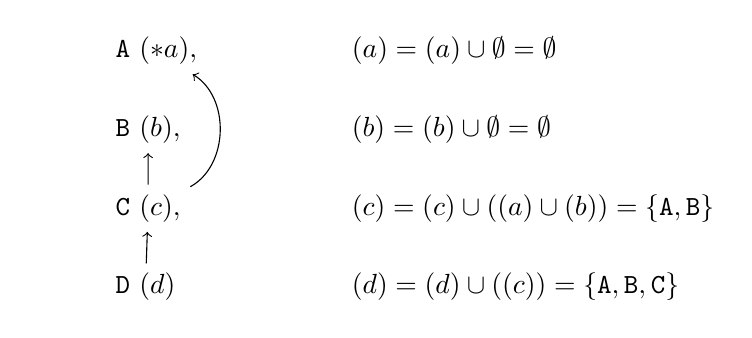
\begin{tikzpicture}[x=10mm, y=10mm]
    \node[anchor=west] at (-1, 0) {\WITH};
    \node[anchor=west] (A) at (0, 0)  {\texttt{A} \AS $(\ast a),$};
    \node[anchor=west] (B) at (0, -1) {\texttt{B} \AS $(b),$};
    \node[anchor=west] (C) at (0, -2) {\texttt{C} \AS $(c),$};
    \node[anchor=west] (D) at (0, -3) {\texttt{D} \AS $(d)$};
    \node[anchor=west] (Ar) at (3, 0)  {$\refs(a) = \FV(a) \cup \emptyset = \emptyset$};
    \node[anchor=west] (Br) at (3, -1) {$\refs(b) = \FV(b) \cup \emptyset = \emptyset$};
    \node[anchor=west] (Cr) at (3, -2) {$\refs(c) = \FV(c) \cup (\refs(a) \cup \refs(b)) = \{\texttt{A}, \texttt{B}\}$};
    \node[anchor=west] (Dr) at (3, -3) {$\refs(d) = \FV(d) \cup (\refs(c)) = \{\texttt{A}, \texttt{B}, \texttt{C}\}$};
    \draw[->, bend right=60] (C) to (A);
    \draw[->] (C) to (B);
    \draw[->] (D) to (C);
    \end{tikzpicture}
    \caption{References are tracked incrementally by collecting free table-variables (ie. direct CTE references) along with the references of those free table-variables.}
    \label{fig:my_label}
\end{figure}


\begin{wrapfigure}{r}{0.5\textwidth}
    \begin{minted}[autogobble]{sql}
        WITH T AS (SELECT 1)
        SELECT *
        FROM (
          WITH T AS (SELECT 2)
          SELECT * FROM T
        ) T
    \end{minted}
    \caption{The outer CTE \texttt{T} is shadowed by an inner CTE. The result of the query is \texttt{2}.}
    \label{lst:indirect_callsite_ref}
\end{wrapfigure}
When tracking table-variables within a scope, we may encounter the effect of \textit{shadowing}. A newly declared variable overrides an existing one of the outer scope. This is an important effect we need to take care of when tracking recursive table variables. \mintinline{psql}{SELECT (SELECT T.v FROM (SELECT f(n-1)) AS T(v)) FROM (SELECT 1) AS T(v)}. The row-reference \texttt{T(v)} is first declared (nonrecursivly) by the outer query and the overridden by the inner query inside \SELECT with a new, recursive definition.


\begin{figure}[h]
    \centering
    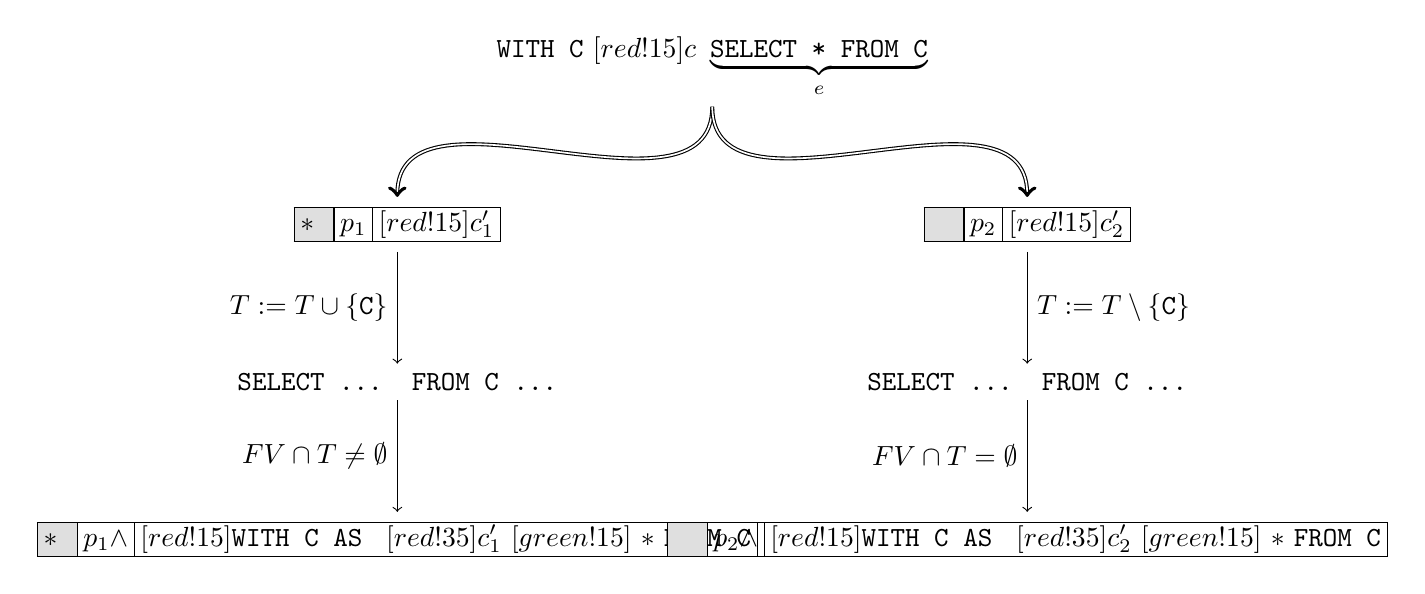
\begin{tikzpicture}
    \node (cte) at (4, 1) {\texttt{WITH C} \AS $\highlight[red!15]{c}~ \underbrace{\texttt{SELECT * FROM C}}_e$};
    \node (cte1) at (0, -1) {
        \begin{tabular}{|p{1em}|r|c|}\hline
        \cellcolor{gray!25} $\ast$ & $p_1$ & $\highlight[red!15]{c'_1}$\\\hline
        \end{tabular}
    };
    \node (cte2) at (8, -1) {
        \begin{tabular}{|p{1em}|r|c|}\hline
        \cellcolor{gray!25} & $p_2$ & $\highlight[red!15]{c'_2}$\\\hline
        \end{tabular}
    };
    \node (select1) at (0, -3) {\texttt{SELECT ... FROM C ...}};
    \node (select2) at (8, -3) {\texttt{SELECT ... FROM C ...}};
    \node (r1) at (0, -5) {
        \begin{tabular}{|p{1em}|r|c|}\hline
        \cellcolor{gray!25} $\ast$ & $p_1 \land \hdots$ & $\highlight[red!15]{\texttt{WITH C AS } ~\highlight[red!35]{c'_1}}~\highlight[green!15]{\SELECT~*~\texttt{FROM C}}$\\\hline
        \end{tabular}
    };
    \node (r2) at (8, -5) {
        \begin{tabular}{|p{1em}|r|c|}\hline
        \cellcolor{gray!25} & $p_2 \land \hdots$ & $\highlight[red!15]{\texttt{WITH C AS } ~\highlight[red!35]{c'_2}}~\highlight[green!15]{\SELECT~*~\texttt{FROM C}}$\\\hline
        \end{tabular}
    };
    \draw[->, double, out=270, in=90] (cte) to (cte1.north);
    \draw[->, double, out=270, in=90] (cte) to (cte2.north);
    \draw[->] (cte1.south) --node[left] {$T := T \cup \{\texttt{C}\}$} (select1);
    \draw[->] (cte2.south) --node[right]{$T := T \setminus \{\texttt{C}\}$} (select2);
    \draw[->] (select1) --node[left] {$FV \cap T \neq \emptyset$} (r1);
    \draw[->] (select2) --node[left] {$FV \cap T = \emptyset$} (r2);
    \end{tikzpicture}
    \caption{}
    \label{fig:my_label}
\end{figure}

The major difference to the \REXPR-rule is that new table-variables are introduces by \FROM, possibly shadowing out outer recursive tables. To reflect this behaviour, we remove all entries from $T$ that are shadowed by the newly introduced table-variables and add those of the newly introduces tables, that are recursive.
But there is one more thing we have to consider: By the fact that the \FROM-part introduces at least one recursive table-variable that is most likely used within \SELECT or \WHERE of the query, we would find out that those parts of the query are also recursive (since they referece a recursive table), violating the overall constraints and rendering the \FROM-rule useless. To avoid this, it is crucial to remove the shadowed table-variables from $T$ but not adding the newly recursive table-variables when checking if \SELECT and \WHERE have a callsite. This way, we allow only referencing only recursive tables introduces by this very query, but forbid any other recursive references.
\sqlcode{snippets/from_shadowing.sql}
\iffalse OLD
$$\quad(\textsc{from})\inferrule{
    \exists i \in \{1, ..., n\}: T \vdash \hasCallsite(e_{f_i}) \\
    T[a_1 \mapsto \bot, ..., a_n \mapsto \bot] \vdash \neg \hasCallsite(e_s) \land \neg \hasCallsite(e_w) \\
    \forall i \in \{1, ..., n\}: T, \varnothing \vdash (\TRUE, t_i) \rightarrow (B_i, R_i)
}{
    T, \varnothing \vdash (p, \SELECT e_s \FROM t_1 \AS a_1 \otimes ... \otimes  t_n \AS a_n \WHERE e_w) \rightarrow \\\\
    {\begin{tabular}[b]{LLLL}
    (~~&\{&(&\SELECT p ~\AND~ p_1 ~\AND~ \cdots ~\AND~ p_n, \\
          &&&\SELECT e_s \FROM t'_1 \AS a_1 \otimes ... \otimes  t'_n \AS a_n \WHERE e_w ~~)\\
      && | &~((p_1, t'_1), ..., (p_n, t'_n)) \in \times_{\{i|1\leq i \leq n\}} B_i\}, \\
    &\{&(&\SELECT p_1 ~\AND~ \cdots ~\AND~ p_n, \\
       &&&\SELECT e_s \FROM t'_1 \AS a_1 \otimes ... \otimes  t'_n \AS a_n \WHERE e_w ~~)\\
       &&| &~ ((p_1, t'_1), ..., (p_n, t'_n)) \in \times_{\{i|1\leq i \leq n\}} (B_i \cup R_i), \exists t' \in \{t'_1, ..., t'_n\} : \hasCallsite(t')\})\\
    \end{tabular}}
}$$
\fi
$$\quad(\textsc{from})\inferrule{
    \exists i \in \{1, ..., n\}: \hasCallsite(T, e_{f_i}) \\
    \neg \hasCallsite(T, e_s)\\
    \neg \hasCallsite(T, e_w) \\\\
    \forall i \in \{1, ..., n\}: T, \varnothing \vdash (\TRUE, t_i) \rightarrow (B_i, R_i)
}{
    T, \varnothing \vdash (p, \SELECT~ e_s ~\FROM~ t_1 \AS a_1 \otimes ... \otimes  t_n \AS a_n ~\WHERE~ e_w) \rightarrow \\\\
    {\begin{tabular}[b]{LLLL}
    (~~&\{&(&\SELECT~ p ~\AND~ p_1 ~\AND~ \cdots ~\AND~ p_n, \\
          &&&\SELECT~ e_s ~\FROM~ t'_1 \AS a_1 \otimes ... \otimes  t'_n \AS a_n ~\WHERE~ e_w ~~)\\
      && | &~((p_1, t'_1), ..., (p_n, t'_n)) \in \times_{\{i|1\leq i \leq n\}} B_i\}, \\[6pt]
    &\{&(&\SELECT~ p_1 ~\AND~ \cdots ~\AND~ p_n, \\
       &&&\SELECT~ e_s ~\FROM~ t'_1 \AS a_1 \otimes ... \otimes  t'_n \AS a_n ~\WHERE~ e_w ~~)\\
       &&| &~ ((p_1, t'_1), ..., (p_n, t'_n)) \in \times_{\{i|1\leq i \leq n\}} (B_i \cup R_i), \exists t' \in \{t'_1, ..., t'_n\} : \hasCallsite(t')\}\\
    )\\
    \end{tabular}}
}$$

\subsection{\RCTE-rule: Collecting and analyzing CTE-Scenarios}
CTE-Scenarios are computed and dependencies for the scenarios are collected.
$$\quad(\textsc{cte})\inferrule{
    \hasCallsite(T, \WITH a_1 \AS t_1, ..., a_n \AS t_n~q)\\
    T, \varnothing \vdash (p, t_1) \rightarrow (B, R) \\
    ((B \times \{\bot\}) \cup (R \times \{\top\})) = \{(p'_{t_1}, t'_1, r_{i_1}), ..., (p'_{t_k}, t'_k, r_k)\} = X\\
    \forall (p'_t, t', r_i) \in X: T[a_1 \mapsto r_i], C[a_1: (t', p'_t, FV^+(t')] \vdash (p, \WITH a_2 \AS t_2, ..., a_n \AS t_n~q) \rightarrow (B_i, R_i)
}{
    T, C \vdash (p, \WITH a_1 \AS t_1, ..., a_n \AS t_n~q) \rightarrow ((\cup_{1 \leq i \leq k} B_i), (\cup_{1 \leq j \leq k} R_j)\})
}$$

$$\quad(\textsc{cte})\inferrule{
    T \vdash \hasCallsite(\WITH~ a_1 \AS t_1, ..., a_n \AS t_n~q)\\
    T, \varnothing \vdash (p, t_1) \rightarrow (B, R) \\
    \forall (p'_t, t') \in B: T \setminus \{a_1\}, C[a_1: (t', p'_t, FV^+(t')] \vdash (p, \WITH~ a_2 \AS t_2, ..., a_n \AS t_n~q) \rightarrow (B_i, R_i) \\
    \forall (p'_t, t') \in R: T \cup \{a_1\}, C[a_1: (t', p'_t, FV^+(t')] \vdash (p, \WITH~ a_2 \AS t_2, ..., a_n \AS t_n~q) \rightarrow (B_j, R_j)
}{
    T, C \vdash (p, \WITH~ a_1 \AS t_1, ..., a_n \AS t_n~q) \rightarrow ((\cup_{1 \leq i \leq k} B_i) \cup (\cup_{1 \leq j \leq l} B_j), (\cup_{1 \leq j \leq k} R_j) \cup (\cup_{1 \leq j \leq l} R_j)\})
}$$

\subsection{\RWITH-rule: Attaching used CTEs only}
When all CTEs at a level are processed, the actual query is processed independently. The query contains none of the preceeding CTEs anymore, so that it is sufficient to analyze the current subtree together with the set $T$ of recursive CTEs in scope to decide whether a subtree is recursive.
$$\quad(\textsc{with})\inferrule{
    C \neq \varnothing\\
    T, \varnothing \vdash (p, q) \rightarrow (B, R)
}{
    T, C \vdash (p, \WITH q) \rightarrow \\\\
    {\begin{tabular}[b]{LLLL}
    (~~&\{&(&\WITH [a_i \AS t_i]^{(a_i, t_i) \in \sigma_{a, t}(q'_{ctePreds})}~\SELECT (\AND_{p_i \in \{p_q\} \cup \sigma_p(q'_{ctes})} p_i), \\
          &&&\WITH [a_i \AS t_i]^{(a_i, t_i) \in \sigma_{a, t}(q'_{ctes})}~~q'~\\
          &&| &~(p_q, q') \in B,~ q'_{ctes} = C[FV^+(q')],~ q'_{ctePreds} = C[\cup_{x_p \in \{p_q\} \cup \sigma_p(q'_{ctes})} FV^+(x_p)]\},\\
    &\{&(&\WITH [a_i \AS t_i]^{(a_i, t_i) \in \sigma_{a, t}(q'_{ctePreds})}~\SELECT (\AND_{p_i \in \{p_q\} \cup \sigma_p(q'_{ctes})} p_i), \\
    &&&\WITH [a_i \AS t_i]^{(a_i, t_i) \in \sigma_{a, t}(q'_{ctes})}~~q'~\\
    &&|&~(p_q, q') \in R,~ q'_{ctes} = C[FV^+(q')],~ q'_{ctePreds} = C[\cup_{x_p \in \{p_q\} \cup \sigma_p(q'_{ctes})} FV^+(x_p)])
    \end{tabular}}
}$$
\\



\section{Postprocessing of the scenarios}
\subsection{Extraction of callsite-arguments}
We need to extract the arguments of the callsites within a recursive case, eg: 
\begin{minted}{sql}
SELECT T.a + T.b + T.c FROM (SELECT f(n-1, 2), 3, 4 + f(5, 6) FROM T WHERE p) AS T(a, b, c)
\end{minted}
into a set of callsite-arguments with its arguments $\{(\SELECT n-1, \SELECT 2), (\SELECT 5, \SELECT 6)\}$. As we require the callsite-arguments to be uncorrelated, we do not have to deal with references to \FROM but only to CTEs, wich simplifies things greatly.

Remove sourrinding query if callsite is within \SELECT, because the value of the callsite-arguments must be invariant to the tables references in \FROM.
$$\quad(\textsc{select})\inferrule{
    \exists i \in \{1, ..., n\}: \text{containsCallsite}(s_i) \\
    \forall i \in \{1, ..., n\}: \varnothing \vdash s_i \rightarrow P_i
}{
    \varnothing \vdash \SELECT s_1, ..., s_n \FROM f \WHERE w \rightarrow \\\\
    \{(\SELECT e_1, ..., \SELECT e_k) | (e_1, ..., e_k) \in \cup_{i \in \{1, ..., n\}} P_i \}
}$$

Remove outer query if callsite is within FROM, because sourrounding query is irrelevant for evaluation of subqueries in FROM.
$$\quad(\textsc{from})\inferrule{
    \forall i_j \in \{i_1, ...., i_m\} \subseteq \{1, ..., n\}: \text{containsCallsite}(f_{i_j})\\
    \forall i_j \in \{i_1, ...., i_m\}: \varnothing \vdash f_{i_j} \rightarrow P_{i_j}
}{
    \varnothing \vdash \SELECT s \FROM a_1 \AS f_1 \otimes ... \otimes a_n \AS f_n \WHERE w \rightarrow \cup_{i \in \{1, ..., n\}} P_i
}$$

Evaluate CTEs seperately, keeping previous CTEs that are referenced, in the case that there are callsites inside CTEs. Saving also every CTE to the CTE-store if they are references form the actual query.
$$\quad(\textsc{cte})\inferrule{
    \varnothing \vdash t_1 \rightarrow P \\
    C[a_1 : (t_1, FV^+(C, t_1))] \vdash \WITH a_2 \AS t_2, ..., a_n \AS t_n ~q \rightarrow P_w
}{
    C \vdash \WITH a_1 \AS t_1, ..., a_n \AS t_n ~q \rightarrow \\\\
    \{(\WITH [a_i \AS t_i]_{(a_i, t_i) \in C[FV^+(e_1)]} ~e_1, ..., \WITH [a_i \AS t_i]_{(a_i, t_i) \in C[FV^+(e_m)]} ~e_m) | (e_1, ..., e_m) \in P\} \cup P_w
}$$


$$\quad(\textsc{with})\inferrule{
    \varnothing \vdash q \rightarrow P
}{
    C \vdash \WITH q \rightarrow \\\\
    \{(\WITH [a_i \AS t_i]_{(a_i, t_i) \in C[FV^+(e)]} ~e_1, ..., \WITH [a_i \AS t_i]_{(a_i, t_i) \in C[FV^+(e_m)]} ~e_m) | (e_1, ..., e_m) \in P\}
}$$

Remove surrounding expression for every branch that contains a callsite, collecting results of all arguments.
$$\quad(\textsc{expr})\inferrule{
    \exists i \in \{1, ...., n\}: \text{containsCallsite}(e_i)\\
    \forall i \in \{1, ...., n\}: \varnothing \vdash e_i \rightarrow P_i
}{
    \varnothing \vdash \text{expr}(e_1, e_2, ..., e_n) \rightarrow \cup_{i \in \{1, ...., n\}} P_i
}$$

Remove recursive call and collect args.
$$\quad(\textsc{call})\inferrule{
}{
    \varnothing \vdash fn_{rec}(e_1, e_2, ..., e_n) \rightarrow \{ (e_1, e_2, ..., e_n) \}
}$$

If subbranch contains no callsite, stop and return empty set.
$$\quad(\textsc{nocall})\inferrule{
\neg \text{containsCallsite}(e)
}{  
    \varnothing \vdash e \rightarrow \{\}
}$$

Callsites within aggregate-functions are forbidden by the restriction that there must be a static number of callsites. Looping through a table, evaluating a recursive call per row is not allowed.



\chapter{Translation Templates}

\section{Callstack discovery}

\begin{minted}{SQL}
SELECT callsite_id, evaluate_arg_1_with_params(params)
FROM predicate_of(scenario) AS p(v)
WHERE p.v
\end{minted}
\section{Callstack evaluation}

\section{Result selection}

\section{Handling nontermination}
Semantic equivalence requires the translation not only to return the same correct results, but also to behave equally in terms of (non)termination. Without special measures, our template will terminate returning a NULL value where the original function 
\subsection{Infinite callstack}
n-1, n-2, n-3, ... looping behaviour is same, callstack table grows forever

\subsection{Looping calls}
n-1, n-1, ... callstack table is finite => but no basecases are reached and evaluation will not start => force loop.

\subsection{Some basecases not reachable}
If only a part of the functions leads to looping calls, evaluation starts since there are basecases, but no final result can be outputted. Force loop.

\chapter{Optimizations}
\section{Handling unhashable types}
\subsection{Detection}
\subsection{Template optimization}

\section{Constant parameter removal}
\subsection{Detection}
\subsection{Template optimization}

\section{Tail Recursion}
\subsection{Detection}
If the result of a recursive call is not used for further computations, ie. the computation context can be disposed, the call is a tail call. If all recursive calls are tail calls, the function is tail recursive. We can utilize this property to skip the evaluation phase which computes the results of all expressions containing a recursive call. In the case of tail recursion the recursive expression equals the call itself, thus no evaluation is required. Usually, the evaluation-phase computes the result of a call with given input parameters by waiting for the results of the callsites and then compute the result of this function call by evaluating the recursive expression with the calls replaced by its results.

A tail recursive function do not need this evaluation phase, because there is no context that need to be evaluated. The context in question is the very call itself. Therefore it is possible to skip the evaluation phase and return directly the result of the last call.

We detect tail recursive calls by analyzing the structure of the recursive cases returned by the static analysis. The only possible strucutre of a tail recursive call is the following
\begin{minted}{SQL}
SELECT (SELECT (SELECT f(..)))
\end{minted}
A complete Example:
\sqlcode{snippets/udf_gcd.sql}

Any computations like \texttt{1+(SELECT f(n))} would create a context around the call that need to be evaluated. The same for \FROM, even if the callsite-arguments contain no table-references, we are required to loop through the rows and create the output table.

If a function is a tail call but its argument references a CTE and therefore the query is prefixed by an \WITH-block, it is still tail recursive, because the reference to any CTE is within the callsite arguments that are removed alltogether with the call during evaluation. So, during evaluation time, the CTEs are not used and thus could be removed, and the expression is tail recursive.
\subsection{Template optimization}

\section{Single Recursion}
\subsection{Detection}
\subsection{Template optimization}
Simple: only one callsite per 
Only one callsite => no need to wait for all callsites of a recursive call
no need to collect all callsites of a given recursive call
union all -> union...wieso?